\section{\name: Bounded Priority Fairness}
\label{sec:impl}

%In this section, we provide a high-level overview of {\name}, which aims at a balance on the potentially conflicting properties. 
%Please refer to our technical report \cite{tech_report} for details. 

\subsection{Modeling the Problem}\label{sec:settings}
% system resource
We consider a system with $K$ types of resources. The capacity of resource $k$ is denoted by $C^k$. The system resource capacity is therefore a vector $\myvec{C} = \langle C^1, C^2, ..., C^K \rangle.$

{\burstq}-$i$'s demand comes from a series $N_i$ of bursts, each consisted of a number of jobs. We denote by $T_i(n)$ the arrival time of the $n$-th burst, which must be finished within $t_i(n)$. Therefore, its $n$-th burst needs to be completed by $T_i(n)+t_i(n)$ (i.e., deadline).
Denote the demand of its $n$-th arrival by a vector $\myvec{d_i}(n)=\langle d^1_i(n), d^2_i(n), ..., d^K_i(n)\rangle$, where $d^k_i(n)$ is the demand on resource-$k$.
We assume users report their estimated demand for presentation simplicity, but uncertainty handling and other details can be found in our technical report~\cite{tech_report}. 



\emph{Completion time:}
Let us denote by $R_i(n)$ the (last) completion time of jobs during {\burstq}-$i$'s $n$-th arrival. If {\burstq}-$i$ is admitted with \emph{hard} guarantee, we ensure that a large fraction ($\alpha_i$, e.g., 95\% or 99\% depending on the SLAs) of arrivals are completed before deadlines, i.e., $\sum_{n\in N_i}\mathbf{1}_{\left\{R_i(n)\leq T_i(n)+t_i(n)\right\}} \geq \alpha_i|N_i|$, where $\mathbf{1}_{\left\{\cdot\right\}}$ is the indicator function.% which equals to 1 if the condition is satisfied and 0 otherwise, $|N_i|$ is the number of arrivals of {\burstq}-$i$. 
If {\burstq}-$i$ is admitted with only \emph{soft/best-effort} guarantee, we want to maximize the fraction of arrivals completed on time.

\emph{Long-term fairness:}
Denote by $\myvec{a_i}(t)$ and $\myvec{e_j}(t)$ the resources allocated for {\burstq}-$i$ and {\batchq}-$j$ at time $t$, respectively.
For a possibly long evaluation interval $[t, t+T]$ during which there is no new admission or exit, the average resource guarantees received are calculated as $\frac{1}{T}\int_t^{t+T} \myvec{a_i}(\tau)\text{d}\tau$ and $\frac{1}{T}\int_t^{t+T} \myvec{e_j}(\tau)\text{d}\tau$.
We require the allocated dominant resource, i.e., the largest amount of resource allocated across all resource types, received by any {\batchq} queue is no smaller than that received by an {\burstq} for isolation protection. %Formally, 

\vspace{-0.1in}	
\subsection{Solution Approach}
\label{sec:solution_approach}

\name consists of the following three major components:

\noindent\textbf{Admission control procedure:} 
\name classifies admitted {\burstq}s and {\batchq}s into three classes: {\burstq}s admitted with hard resource guarantee ($\mathbb{H}$), {\burstq}s admitted with soft resource guarantee ($\mathbb{S}$), and elastic queues that can be either {\burstq}s or {\batchq}s ($\mathbb{E}$).

Before admitting \burstq-$i$, \name checks if admitting it invalidates any resource guarantees committed for {\burstq}s in $\mathbb{H}\cup\mathbb{S}$, i.e., the \emph{safety condition} $\myvec{d_j}(n) \leq \frac{\myvec{C}\left(T_j(n+1)-T_j(n)\right)}{|\mathbb{H}|+|\mathbb{S}|+|\mathbb{E}|+1}, \forall n, \forall j \in \mathbb{H}\cup\mathbb{S}$.
If it is not satisfied, \burstq-$i$ is rejected. Otherwise, it is safe to admit \burstq-$i$. If its own total demand exceeds its long-term fair share (\emph{fairness condition}), \burstq-$i$ is added to $\mathbb{E}$ for best-effort services. Otherwise if there are enough uncommitted resources, \burstq-$i$ is added to $\mathbb{H}$ with hard guarantee. If there are not enough resources left, it is added to $\mathbb{S}$. 
For {\batchq}-$j$, \name simply checks the safety condition. If it is satisfied, {\batchq}-j is added to $\mathbb{E}$. Otherwise {\batchq}-$j$ is rejected.


\noindent\textbf{Guaranteed resource provisioning procedure}: 
For each {\burstq}-$i$ in $\mathbb{H}$, during $[T_i(n),T_i(n)+t_i(n)]$, \name allocates constant resources to fulfill its demand $\myvec{a_i}(t)=\frac{\myvec{d_i}(n)}{t_i(n)}$. %\footnote{In practice, {\burstq}-$i$ may not fully receive the guaranteed resources. For instance, non-preemption settings do not allow the cluster to kill the running jobs or tasks to give more resources to {\burstq}-$i$ immediately at the beginning of its burst. In such cases, more resources may be provided to {\burstq}-$i$ during the OFF period $[T_i(n)+t_i(n),T_i(n+1)]$ until its resource consumption reaches $\myvec{d_i}(n)t_i(n)$.}. 
{\burstq}s in $\mathbb{S}$ shares the uncommitted resource $\myvec{C}-\sum_{j\in \mathbb{H}}\myvec{a_j}(t)$ based on SRPT~\cite{bansal2001analysis} until each {\burstq}-$i$'s consumption reaches $\myvec{d_i}(n)$ or the deadline arrives. 
Remaining resources are allocated to queues in $\mathbb{E}$ using DRF~\cite{drf}. %\nhattan{do we really need this? It is the same as in Spare resource scheduling.}


\noindent\textbf{Spare resource allocation procedure}:
If some allocated resources are not used, they are further shared by {\batchq}s and {\burstq}s with unsatisfied demand. This maximizes system utilization.









\vspace{-0.1in}
\subsection{Properties of \name}

First, we briefly discuss how \emph{\name ensures long-term fairness, burst guarantee, and Pareto efficiency}. 
%Corresponding proofs can be found in the appendix.
%\zhenhua{Xiao, could you please add the proofs? The following paragraphs may be useful.}\xiao{added below,I didn't say much about pareto-efficienncy as in our discussion before, I feel this is enough.} 
The safety condition and fairness condition ensure the long-term fairness for all {\batchq}s. %They have no fewer resources than any {\burstq} in the long-term, so it is beneficial for them to share the resources. 
For {\burstq}s in $\mathbb{H}$, they have hard resource guarantee and therefore can meet their SLA. For {\burstq}s in $\mathbb{S}$, they have resource guarantee whenever possible, and only need to wait after {\burstq}s in $\mathbb{H}$ when there is a conflict. Therefore, their performance is much better than if they were under fair allocation policies. %Therefore, both of them have incentives to share. % both of them reach long-term fairness and sharing incentive.
%^For burst guarantee, it is straightforward from our algorithm that we have the hard guarantee for all {\burstq}s in $\mathbb{H}$, and best-effort guarantee for {\burstq}s in $\mathbb{S}$.
The addition of $\mathbb{S}$ allows more {\burstq}s to be admitted with resource guarantee, and therefore increases the system resources utilized by {\burstq}s. Finally, we fulfill spare resources with {\batchq}s, so system utilization is maximized, reaching Pareto efficiency.

In addition, we prove that \emph{\name is strategyproof} in~\cite{tech_report}.

%We restrict our attention in this paper to the following, important properties: burst guarantee for {\burstq}s, long-term fairness for {\batchq}s, strategyproofness, and Pareto efficiency to improve cluster utilization.
%
%\textbf{Burst guarantee (BG)} provides performance guarantee for {\burstq}s by allocating guaranteed amount of resources during their bursts. 
%In particular, an {\burstq} requests its minimum required resources for its bursts to satisfy its service level agreements, e.g., percentiles of response time. 
%
%\textbf{Long-term fairness (LF)} provides every queue in the system the same amount of resources over a (long) period, e.g., 10 minutes.
%Overall, it ensures that {\batchq}s progress no slower than any {\burstq} in the long run. LF implies sharing incentive, which requires that each queue should be better off sharing the cluster, than exclusively using its own static share of the cluster. 
%If there are $n$ queues, each queue cannot exceed $\frac{1}{n}$ of all resources under a static sharing.\footnote{For simplicity of presentation, we consider queues with the same weights, which can be easily extended to queues with different weights.}
%
%\textbf{Strategyproofness (SPF)} ensures that queues cannot benefit by lying about their resource demands. 
%This provides incentive compatibility, as a queue cannot improve its allocation by lying. 
%
%\textbf{Pareto efficiency (PE)} is about the optimal utilization of the system. 
%A resource allocation is Pareto efficient if it is impossible to increase the allocation/utility of a queue without hurting at least another queue. %This property is important as it leads to maximizing system utilization subject to satisfying the other properties.


\vspace{-0.1in}
\subsection{Enabling \name in Cluster Managers}

We now describe how we have implemented \name on Apache YARN. We use standard techniques for demand estimation.
A key benefit of {\name} is its simplicity of implementation: we have implemented it in YARN using only $600$ lines of code. We made three main changes for user input, admission control, and resource scheduler -- all in the \emph{resource manager} (RM). 
We do not modify \emph{node manager} (NM) or application master (AM). 
Figure~\ref{fig:system_design} depicts our design.
More detailed implementation and operational issues can be found in our full technical report \cite{tech_report}.

\begin{figure}[h]
	\centering
	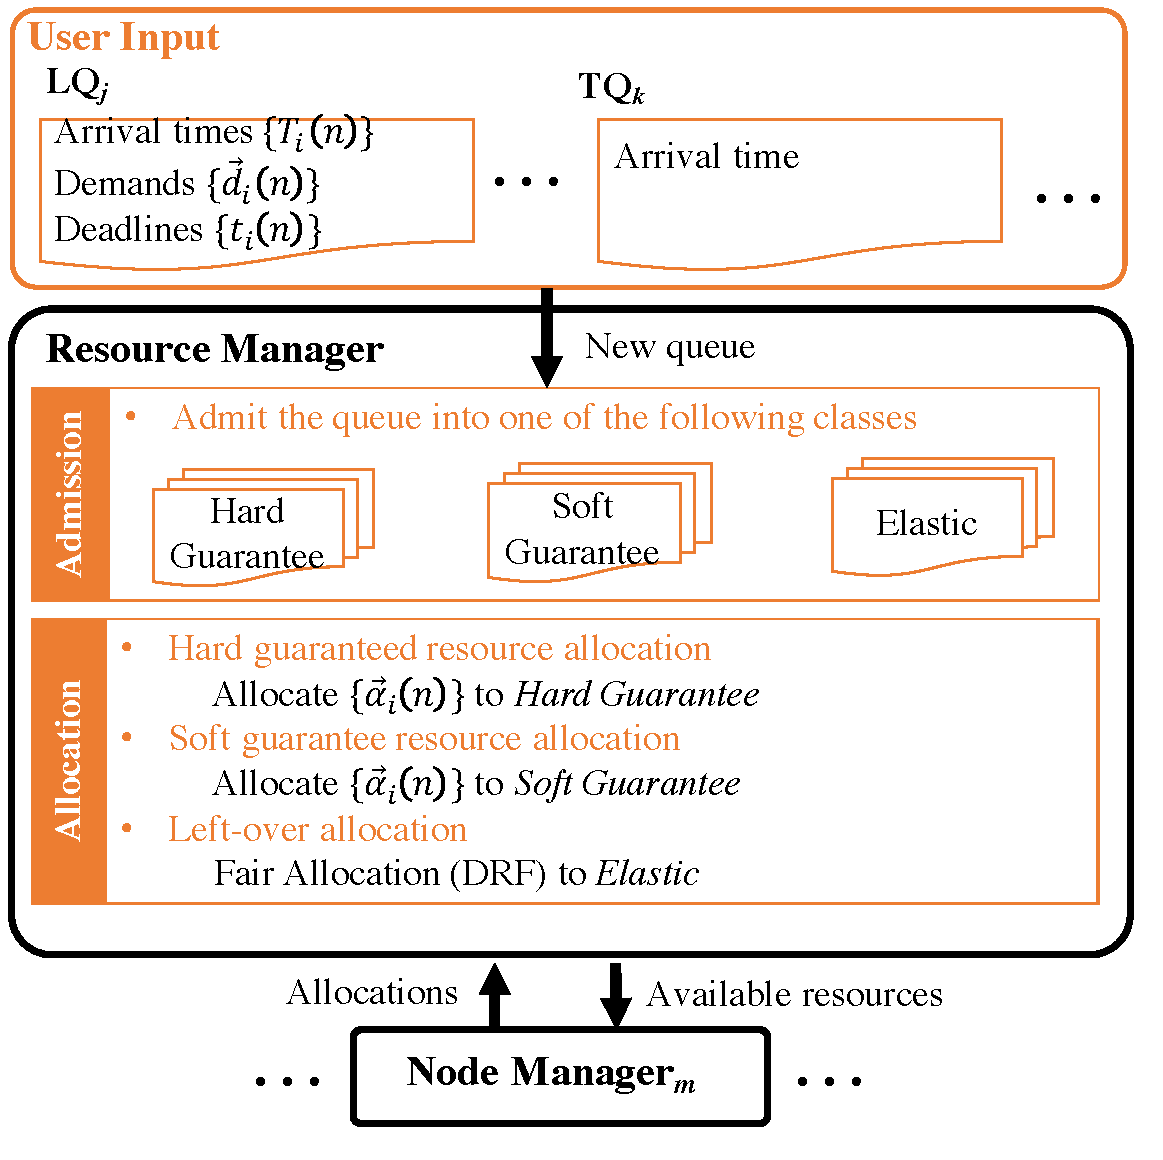
\includegraphics[width=0.8\linewidth]{fig/diagram}
	\vspace{-0.2in}
	\caption{Enabling bounded prioritization with long-term fairness in a  multi-resource cluster.}
	\vspace{-0.2in}
	\label{fig:system_design}
\end{figure}